\documentclass[12pt,a4paper]{report}
\usepackage[utf8]{inputenc}
\usepackage{graphicx}
\usepackage{setspace}
\usepackage{geometry}
\geometry{left=4cm,right=3cm,top=3cm,bottom=3cm}
\onehalfspacing
% \setlength{\textfloatsep}{0pt plus 1.0pt minus 2.0pt}
% \setlength{\floatsep}{0pt plus 1.0pt minus 2.0pt}
% \setlength{\intextsep}{0pt plus 1.0pt minus 2.0pt}
\setlength{\textfloatsep}{15pt plus 2.0pt minus 2.0pt}
\setlength{\floatsep}{12pt plus 2.0pt minus 2.0pt}
\setlength{\intextsep}{12pt plus 2.0pt minus 2.0pt}

\usepackage{fancyhdr}
\pagestyle{fancy}

\usepackage{tocloft}
\usepackage{hyperref}
\usepackage{lipsum}
\usepackage{indentfirst}
\usepackage{newtxtext,newtxmath} % Times New Roman font
\usepackage{sectsty}
\usepackage{tabularx}
\usepackage{caption}
\usepackage{float} % untuk [H] agar posisi tabel tepat di lokasi kode
\usepackage[style=apa,sorting=nyt]{biblatex}
\usepackage{longtable}
\usepackage{array}    % untuk p{width}
\usepackage{caption}  % opsional, agar caption bisa dikustomisasi
\usepackage{lscape} % jika ingin landscape
\usepackage{booktabs}
\usepackage{multirow}
\usepackage[table,xcdraw]{xcolor}
\usepackage{lscape}
\usepackage{chngcntr}
\usepackage{tocloft}
% Hilangkan space sebelum judul daftar isi/gambar/tabel

\renewcommand{\cfttoctitlefont}{}
\renewcommand{\cftloftitlefont}{}
\renewcommand{\cftlottitlefont}{}
\renewcommand{\cftaftertoctitle}{}
\renewcommand{\cftafterloftitle}{}
\renewcommand{\cftafterlottitle}{}

\setlength{\cftbeforetoctitleskip}{0pt}
\setlength{\cftaftertoctitleskip}{0pt}

\setlength{\cftbeforeloftitleskip}{0pt}
\setlength{\cftafterloftitleskip}{0pt}

\setlength{\cftbeforelottitleskip}{0pt}
\setlength{\cftafterlottitleskip}{0pt}

\counterwithin{figure}{chapter} % atau {section} kalau tiap section
\counterwithin{table}{chapter}
\DeclareLanguageMapping{english}{english-apa}
% \DefineBibliographyStrings{english}{andothers = {dkk.,}}
\addbibresource{reference.bib} % file referensi BibTeX

\newcommand{\bab}[2]{
  \refstepcounter{chapter} % Tambahkan ini untuk update counter
  \chapter*{
    \makebox[\textwidth][c]{\textbf{#1}}\\
    \makebox[\textwidth][c]{\textbf{#2}}
  }
  \addcontentsline{toc}{chapter}{#1 #2}
  \setcounter{section}{0} % Reset section tiap bab
}
\renewcommand{\figurename}{Gambar}
\renewcommand{\tablename}{Tabel}
\chapterfont{\normalsize}
\sectionfont{\normalsize}
\subsectionfont{\normalsize}
\subsubsectionfont{\normalsize}
\setcounter{secnumdepth}{4}
\setcounter{tocdepth}{4}
% \renewcommand{\contentsname}{Daftar Isi}       % Ganti judul TOC
% \renewcommand{\listfigurename}{Daftar Gambar}  % Ganti judul daftar gambar
% \renewcommand{\listtablename}{Daftar Tabel}    % Ganti judul daftar tabel
\renewcommand{\contentsname}{}       % Hapus judul default "Daftar Isi"
\renewcommand{\listfigurename}{}     % Hapus judul default "Daftar Gambar"
\renewcommand{\listtablename}{}      % Hapus judul default "Daftar Tabel"

\begin{document}
\fancyhf{}
  \fancyfoot[C]{\thepage}
  \renewcommand{\headrulewidth}{0pt}
  \renewcommand{\footrulewidth}{0pt}
\pagenumbering{gobble}
\begin{titlepage}
    \thispagestyle{empty}
    \begin{center}
        \textbf{\large Arsitektur End-to-End Multitask Learning Berbasis Transformer untuk
        Peningkatan Driving Score Kendaraan Otonom}
    
        \vspace{1.5cm}
    
        \textbf{SKRIPSI}
        \vspace{0.5cm}

        Diajukan sebagai syarat untuk memperoleh gelar Sarjana Komputer \\ Program Studi Ilmu Komputer

        \vspace{2cm}
    
        \includegraphics[width=4cm]{images/image11.png}
    
        \vspace{2cm}
    
        \textbf{OLEH:} \\[0.5cm]
        \textbf{FACHRI NAJM NOER KARTIMAN} \\[0.2cm]
        2106515
    
        \vfill
    
        \textbf{PROGRAM STUDI S1 ILMU KOMPUTER} \\
        \textbf{FAKULTAS PENDIDIKAN MATEMATIKA DAN ILMU PENGETAHUAN ALAM} \\
        \textbf{UNIVERSITAS PENDIDIKAN INDONESIA} \\
        2025
    \end{center}
    \end{titlepage}
    

\clearpage
\pagenumbering{roman}
\setcounter{page}{1}

\bab{ABSTRAK}{}
% \addcontentsline{toc}{section}{ABSTRAK}
\vspace{-1cm}

Perkembangan teknologi kendaraan otonom menuntut sistem perencanaan jalur yang mampu memahami lingkungan secara menyeluruh dan menghasilkan keputusan mengemudi yang akurat dan aman. Model perencanaan tradisional berbasis CNN seringkali memiliki keterbatasan dalam menangkap konteks global dan hubungan antar elemen lingkungan secara efektif. Untuk mengatasi hal tersebut, penelitian ini mengusulkan arsitektur SKGE-Swin yang memanfaatkan Swin Transformer dengan mekanisme skip stage guna memperkuat representasi fitur di berbagai level jaringan. Pendekatan ini memungkinkan model untuk mempertahankan informasi penting dari tahap awal hingga akhir proses ekstraksi fitur, sehingga meningkatkan kemampuan dalam memahami pola kompleks di sekitar kendaraan. Hasil eksperimen menunjukkan bahwa arsitektur SKGE-Swin mampu memberikan performa yang lebih baik dengan Driving Score sebesar 37.10 dalam tugas prediksi waypoint dibandingkan dengan metode CNN, sehingga berkontribusi pada pengembangan sistem kendaraan otonom yang lebih handal dan aman.

\vspace{0.5cm}
\textbf{Kata kunci:} multitask learning, transformer,  Kendaraan otonom, perencanaan jalur, Swin Transformer, skip stage, prediksi waypoint, representasi fitur, model deep learning.


\include{kata_pengantar}

\clearpage
\bab{DAFTAR ISI}{}
\vspace{-1cm}  % sesuaikan nilai ini sampai spasi hilang
\tableofcontents

\clearpage
\bab{DAFTAR GAMBAR}{}
\vspace{-1cm}
\listoffigures

\clearpage
\bab{DAFTAR TABEL}{}
\vspace{-1cm}
\listoftables

\clearpage
\pagenumbering{arabic}
\setcounter{page}{1}
\fancyhf{}

% Nomor halaman di kanan bawah untuk halaman biasa
\fancyhead[R]{\thepage}

\renewcommand{\headrulewidth}{0pt}
% \fancyhead[R]{\thepage}
% \renewcommand{\headrulewidth}{0pt}
% % Atur agar halaman awal bab juga ikut pakai fancy
\fancypagestyle{plain}{
  \fancyhf{}
  \fancyfoot[C]{\thepage}
  \renewcommand{\headrulewidth}{0pt}
  \renewcommand{\footrulewidth}{0pt}
}
\bab{BAB I}{PENDAHULUAN}
\setcounter{chapter}{1}

\renewcommand{\thesection}{\thechapter.\arabic{section}}
\section{Latar Belakang}

Kendaraan otonom telah menjadi salah satu inovasi teknologi paling menjanjikan dalam sektor transportasi modern. 

\begin{figure}[H]
    \centering
    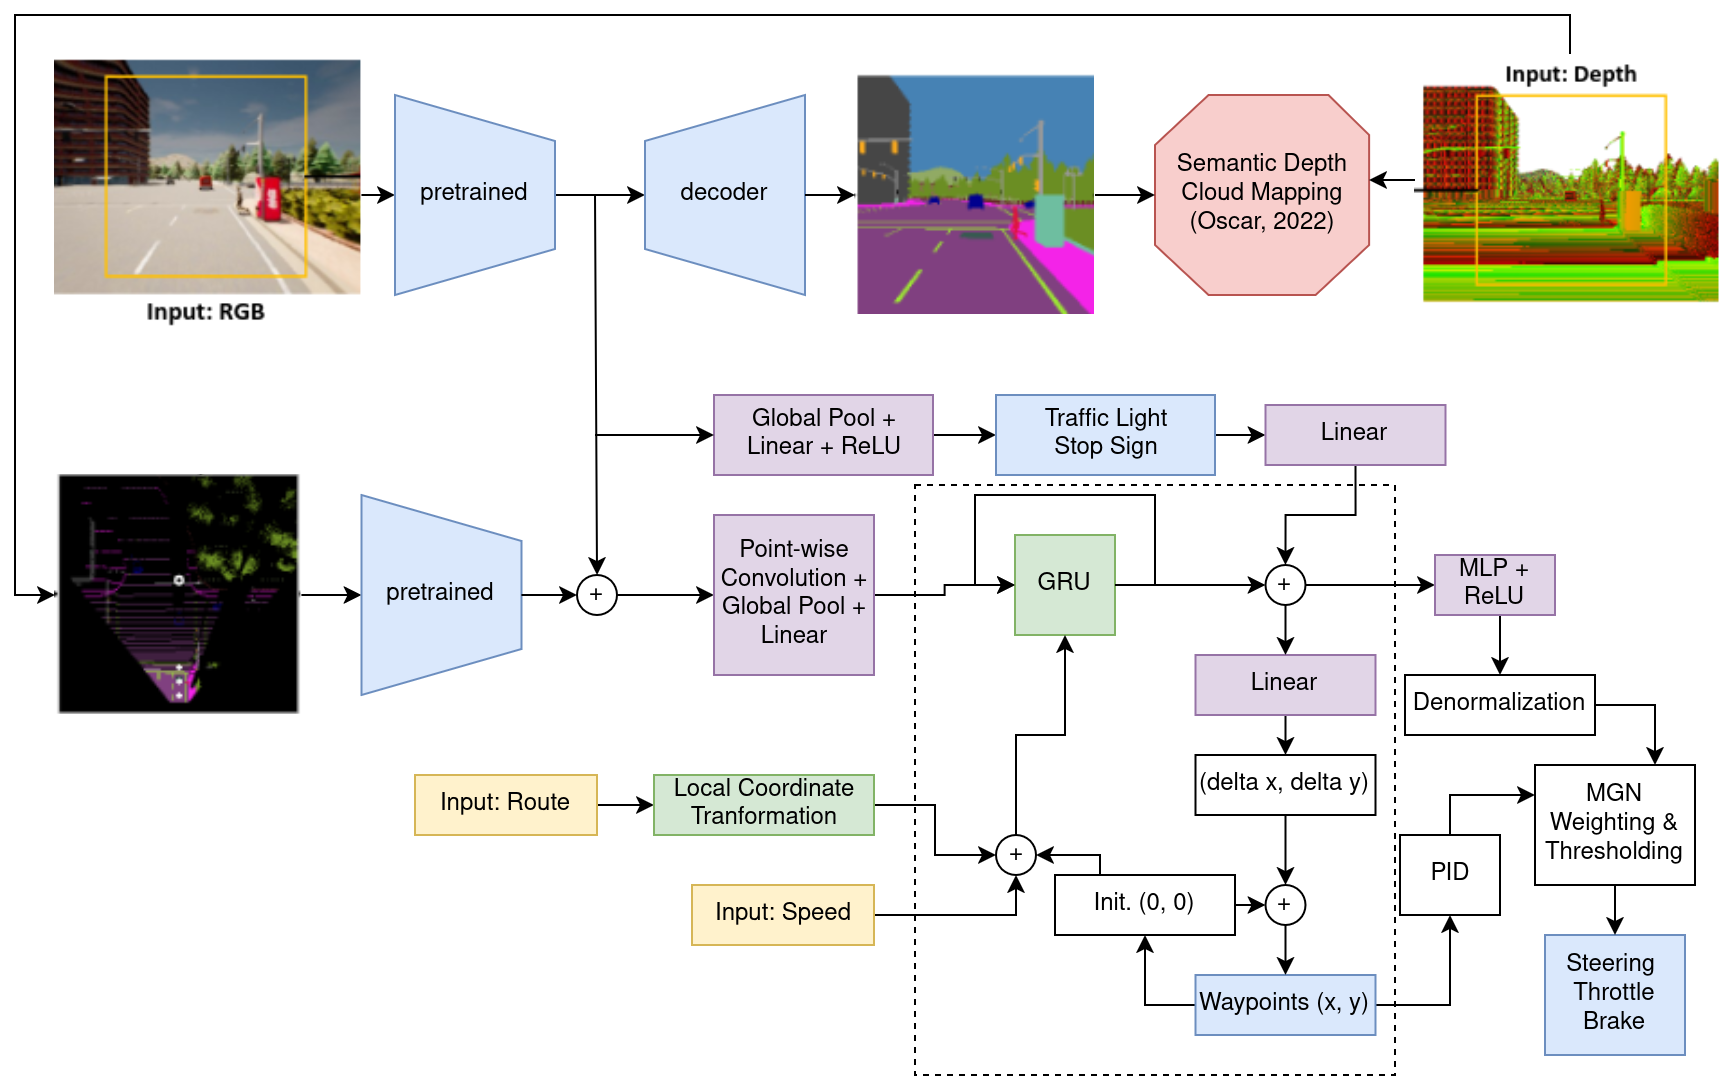
\includegraphics[width=1\textwidth]{images/architecture-x13.png}
    \caption{Arsitektur x13 \parencite{Natan2023-hi}.}
    \label{fig:architecture_x13}
\end{figure}

Pada Gambar \ref{fig:architecture_x13}, ditampilkan arsitektur x13 yang digunakan dalam sistem prediksi waypoints dan navigasi kendaraan otonom. Arsitektur ini terdiri dari beberapa komponen utama, termasuk EfficientNet sebagai backbone untuk ekstraksi fitur dari input RGB, Gated Recurrent Unit (GRU) untuk memproses data sekuensial dan menghasilkan prediksi waypoints, serta encoder untuk ekstraksi fitur dari semantic depth cloud. Dalam arsitektur ini, input berupa gambar RGB dan data kedalaman (depth) diproses melalui modul segmentasi untuk menghasilkan peta kedalaman semantic depth cloud (SDC), yang kemudian digunakan dalam proses pengambilan keputusan terkait navigasi.

\section{Rumusan Masalah}
\begin{enumerate}
    \item Bagaimana pemanfaatan arsitektur Transformer dalam komponen arsitektur berbasis CNN tradisional, seperti EfficientNet dan GRU, untuk meningkatkan performa prediksi waypoints dan navigasi pada kendaraan otonom?
    \item Apakah penggunaan Transformer mampu meningkatkan akurasi dan responsivitas sistem kendaraan otonom terhadap perubahan kondisi jalan yang dinamis?
    \item Apa saja kendala teknis yang muncul dalam penerapan arsitektur Transformer, khususnya terkait kebutuhan komputasi dan dataset pelatihan pada tugas multi-task learning untuk kendaraan otonom?
\end{enumerate}

\section{Batasan Masalah}
Dalam penelitian ini, terdapat beberapa batasan yang perlu diperhatikan untuk memperjelas ruang lingkup dan fokus studi yang akan dilakukan, antara lain:
\subsection{
    Lingkup Data Sensor yang Digunakan
}
Penelitian ini akan menggunakan data dari sensor kamera RGB-D dan informasi lokasi dari GPS untuk proses persepsi lingkungan dan pengambilan keputusan. Data dari sensor tambahan seperti LiDAR atau radar tidak akan dipertimbangkan dalam penelitian ini, sehingga hasil penelitian terbatas pada arsitektur yang mengandalkan data visual dan kedalaman dari kamera RGB-D.

\bab{BAB II}{TINJAUAN PUSTAKA}


% \addcontentsline{toc}{chapter}{BAB II TINJAUAN PUSTAKA}
\setcounter{chapter}{2}
\setcounter{section}{0} % RESET section ke 0
\renewcommand{\thesection}{\thechapter.\arabic{section}}
\section{Kendaraan Otonom dan Tantangan dalam Navigasi
}
Penelitian \textcite{Ni2020-oa} menggunakan sensor LIDAR, GPS, IMU untuk mengatasi permukaan jalan yang tidak rata dan mengidentifikasi rintangan di sekitar kendaraan. Dengan memanfaatkan data dari berbagai sensor, sistem kendaraan otonom dapat meningkatkan persepsi lingkungan dan kemampuan navigasi secara signifikan.

\bab{BAB III}{METODE PENELITIAN}


% \addcontentsline{toc}{chapter}{BAB II TINJAUAN PUSTAKA}
\setcounter{chapter}{3}
\setcounter{section}{0} % RESET section ke 0
\renewcommand{\thesection}{\thechapter.\arabic{section}}
Penelitian ini menggunakan metode \parencite{santoso2020implementasi} dalam bentuk eksperimen untuk mengevaluasi model deep learning dalam tugas prediksi waypoint, segmentasi semantik, dan ekstraksi fitur visual pada sistem kendaraan otonom. Pada Gambar \ref{fig:desain_penelitian} dapat dilihat desain penelitian yang digunakan dalam penelitian ini. Penelitian ini bermulai dari  perumusan masalah, kemudian dilanjutkan dengan studi literatur, pengumpulan data, praproses data, perancangan algoritma, pelatihan model, evaluasi model, dan terakhir penarikan kesimpulan.
\vspace{1cm}
\begin{figure}[H]
    \centering
    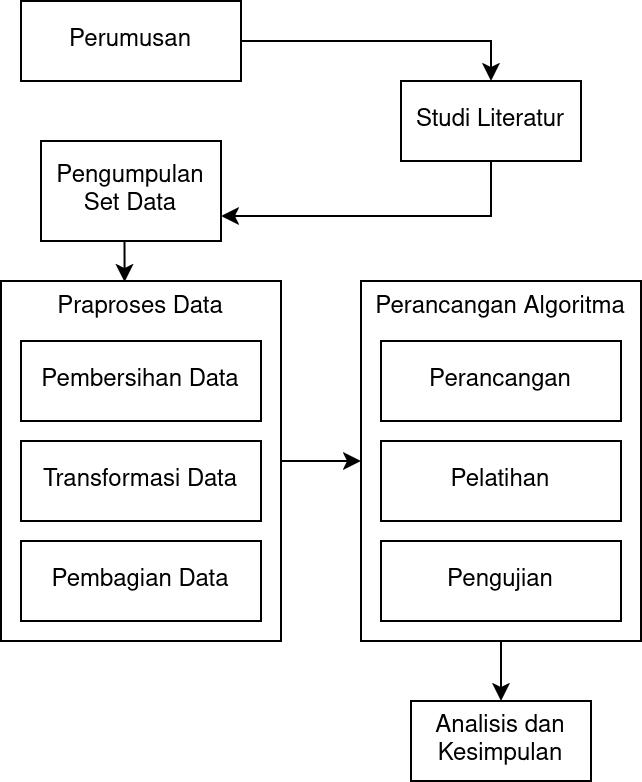
\includegraphics[width=0.6\textwidth]{images/desain-penelitian.png}
    \caption{Desain Penelitian.}
    \label{fig:desain_penelitian}
\end{figure}

\section{Pengumpulan Set Data}

\subsection{Variasi Dataset}
\begin{equation}
    D = \{(X_i, Y_i)\}_{i=1}^{J}
\end{equation}


\subsection{Representasi Data}
\begin{enumerate}
    \item{LiDAR Point Clouds}\\
    Lidar point clouds direpresentasikan sebagai tensor 3D dengan dimensi pada
$
    \mathbb{R}^{4 \times 13716}
$
di mana 4 adalah jumlah fitur (x, y, z, intensitas) dan 13716 adalah jumlah titik yang diambil dari LiDAR. Data point cloud ini memberikan informasi tentang posisi dan intensitas cahaya yang dipantulkan oleh objek di sekitar kendaraan.


    \item{Segmentasi Semantik}\\
\begin{equation}
    R \in \{0, 1\}^{23 \times 256 \times 256}
\end{equation},
    \item{Waypoints}\\
Waypoints dilambangkan sebagai
\begin{equation}
    \omega_i^\rho = (x_i, y_i)
\end{equation}

    \item{Kontrol Kendaraan}\\
    \label{sec:kontrol_kendaraan}

Steering $\in [-1, 1]$

Throttle $\in [0, 0.75]$

Brake $\in [0, 1]$


    \item{Informasi Tambahan}\\
\end{enumerate}


\subsection{Konfigurasi Data CARLA}


\begin{table}[H]
\centering
\caption{Carla Dataset Setting}
\label{tab:carla_dataset_setting}
\begin{tabularx}{\textwidth}{lX}
\hline
\textbf{Maps} & Town01, Town02, Town03, Town04, Town05, Town06, Town07, Town10 \\
\hline
\textbf{Route sets*} & 
Long (1000--200m), Short (100--500m), Tiny (one turn or one go-straight) \\
\hline
\textbf{Weather presets} & ClearNoon \\
\hline
\textbf{Non-playable characters} & Vehicles (truck, car, bicycle, motorbike) and pedestrians \\
\hline
\textbf{Object classes} & 
0: Unlabeled, 1: Building, 2: Fence, 3: Other, 4: Pedestrian, 5: Pole, 6: Road lane, 7: Road, 8: Sidewalk, 9: Vegetation, 10: Other vehicles, 11: Wall, 12: Traffic sign, 13: Sky, 14: Ground, 15: Bridge, 16: Rail track, 17: Guard Trail, 18: Traffic light, 19: Static Object, 20: Dynamic Object, 21: Water, 22: Terrain \\
\hline
\textbf{CARLA version} & 0.9.10.1 \\
\hline
\end{tabularx}
\end{table}
\section{Praproses Data}
\subsection{Pembersihan Data}
\subsection{Transformasi Data}

        Formula yang digunakan untuk mendekode nilai kedalaman adalah sebagai berikut \parencite{carladepthcamera}:
        \begin{equation}
            \mathbb{R}_i^{\text{dec}} = \frac{R_i + 256 G_i + 256^2 B_i}{256^3 - 1} \times 1000,
            \end{equation}
      

\subsubsection{Swin Transformer Varians}
Swin Transformer memiliki beberapa varian yang berbeda, masing-masing dengan karakteristik dan ukuran yang berbeda. Tabel \ref{tab:swin_variants} menunjukkan perbandingan antara varian-varian tersebut, termasuk ukuran patch, dimensi embedding, jumlah layer, jumlah head, jumlah parameter (M), dan FLOPs (G). Setiap varian memiliki keunggulan dan kelemahan masing-masing, sehingga pemilihan varian yang tepat sangat penting untuk mencapai performa yang optimal dalam tugas-tugas tertentu.
\begin{table}[H]
    \centering
    \caption{Varian Swin Transformer dan Karakteristiknya}\label{tab:swin_variants}
    \resizebox{\textwidth}{!}{%
    \begin{tabular}{lccccccp{5cm}}
    \hline
    \textbf{Varian} & \textbf{Patch Size} & \textbf{Dimensi Embed} & \textbf{Jumlah Layer} & \textbf{Jumlah Head} & \textbf{Param (M)} & \textbf{FLOPs (G) @224} & \textbf{Ciri Khas} \\
    \hline
    Swin-T (Tiny)  & 4×4 & 96  & [2, 2, 6, 2]  & [3, 6, 12, 24]  & 28M  & 4.5  & Ringan, cocok untuk device terbatas \\
    Swin-S (Small) & 4×4 & 96  & [2, 2, 18, 2] & [3, 6, 12, 24]  & 50M  & 8.7  & Trade-off antara performa dan ukuran \\
    Swin-B (Base)  & 4×4 & 128 & [2, 2, 18, 2] & [4, 8, 16, 32]  & 88M  & 15.4 & Performansi tinggi, sering dipakai \\
    Swin-L (Large) & 4×4 & 192 & [2, 2, 18, 2] & [6, 12, 24, 48] & 197M & 34.5 & Sangat kuat, untuk tugas kompleks \\
    \hline
    \end{tabular}%
    }
    \end{table}
    


\subsection{Evaluasi}
\bab{BAB IV}{HASIL DAN PEMBAHASAN}


% \addcontentsline{toc}{chapter}{BAB II TINJAUAN PUSTAKA}
\setcounter{chapter}{4}
\setcounter{section}{0} % RESET section ke 0
\renewcommand{\thesection}{\thechapter.\arabic{section}}
\begin{table}[]
    \centering
    \caption{Desain Eksperimen Waypoint}
    \label{tab:waypoint-desain-eksperimen}
    \begin{tabular}{ll}
    \toprule
    \textbf{Model} & \textbf{Menggunakan} \\
    \midrule
    x13t & Transformer \\
    cx13 & Cross Attention + GRU \\
    \bottomrule
    \end{tabular}
\end{table}
\bab{BAB V}{KESIMPULAN DAN SARAN}


% \addcontentsline{toc}{chapter}{BAB II TINJAUAN PUSTAKA}
\setcounter{chapter}{5}
\setcounter{section}{0} % RESET section ke 0
\renewcommand{\thesection}{\thechapter.\arabic{section}}

\bab{DAFTAR PUSTAKA}{}
\defbibheading{none}{} % <-- Hapus heading default
\renewcommand*{\bibfont}{\normalfont\small\onehalfspacing}
\setlength{\bibhang}{1cm}
\printbibliography[heading=none]% Menampilkan daftar pustaka

\end{document}
